%%%%%%%%%%%%%%%%%%%%%%%%%%%%%%%%%%%%%%%%%
% Masters/Doctoral Thesis
% LaTeX Template
% Version 2.5 (27/8/17)
%
% This template was downloaded from:
% http://www.LaTeXTemplates.com
%
% Version 2.x major modifications by:
% Vel (vel@latextemplates.com)
%
% This template is based on a template by:
% Steve Gunn (http://users.ecs.soton.ac.uk/srg/softwaretools/document/templates/)
% Sunil Patel (http://www.sunilpatel.co.uk/thesis-template/)
%
% Template license:
% CC BY-NC-SA 3.0 (http://creativecommons.org/licenses/by-nc-sa/3.0/)
%
%%%%%%%%%%%%%%%%%%%%%%%%%%%%%%%%%%%%%%%%%

%%%%%%%%%%%%%%%%%%%%%%%%%%%%%%%%%%%%%%%%%
% José Miguel García Benayas
% Universidad Rey Juan Carlos
% Móstoles Madrid España
% Escuela Técnica Superior de Ingeniería Informática
% Grado en Ingeniería del Software
% 2019
%%%%%%%%%%%%%%%%%%%%%%%%%%%%%%%%%%%%%%%%%

%-------------------------------------------------------------------------------
%	PACKAGES AND OTHER DOCUMENT CONFIGURATIONS
%-------------------------------------------------------------------------------

\documentclass[
12pt, % The default document font size, options: 10pt, 11pt, 12pt
%oneside, % Two side (alternating margins) for binding by default, uncomment to switch to one side
spanish, % ngerman for German
onehalfspacing, % Single line spacing, alternatives: onehalfspacing or doublespacing
%draft, % Uncomment to enable draft mode (no pictures, no links, overfull hboxes indicated)
%nolistspacing, % If the document is onehalfspacing or doublespacing, uncomment this to set spacing in lists to single
%liststotoc, % Uncomment to add the list of figures/tables/etc to the table of contents
%toctotoc, % Uncomment to add the main table of contents to the table of contents
parskip, % Uncomment to add space between paragraphs
%nohyperref, % Uncomment to not load the hyperref package
headsepline, % Uncomment to get a line under the header
%chapterinoneline, % Uncomment to place the chapter title next to the number on one line
%consistentlayout, % Uncomment to change the layout of the declaration, abstract and acknowledgements pages to match the default layout
openany % Uncomment to delete white page after introduction chapter
]{MastersDoctoralThesis} % The class file specifying the document structure

\usepackage[utf8]{inputenc} % Required for inputting international characters
\usepackage[T1]{fontenc} % Output font encoding for international characters

\usepackage{mathpazo} % Use the Palatino font by default
\usepackage{amsmath} % More math functions

\usepackage[backend=bibtex,natbib=true]{biblatex} % Use the bibtex backend with the authoryear citation style (which resembles APA)

\addbibresource{main.bib} % The filename of the bibliography

\usepackage[autostyle=true]{csquotes} % Required to generate language-dependent quotes in the bibliography

\usepackage{listings} % Package to type bash commands

\usepackage{imakeidx} % Package to make an index of words used in the papers

\makeindex[program=makeindex,columns=2,intoc=true,options={-s index_style.ist}]

\usepackage[hidelinks]{hyperref} % Used to hide the link frames

\usepackage[ruled, vlined, spanish, onelanguage, linesnumbered]{algorithm2e} %for psuedo code

\usepackage{rotating} 
\usepackage{schemata}
\newcommand\diagram[2]{\schema{\schemabox{#1}}{\schemabox{#2}}}

\usepackage{graphicx}
\usepackage{float}
\usepackage{subfigure}
\usepackage{amssymb, amsmath, amsbsy} % simbolos
\usepackage{upgreek} % para poner letras griegas sin cursiva

\usepackage[automake]{glossaries} %Load glossaries package
\makeglossaries

\usepackage[bottom]{footmisc}


% Start - Convert csv to table %
\usepackage{booktabs} % For \toprule, \midrule and \bottomrule
\usepackage{siunitx} % Formats the units and values
\usepackage{pgfplotstable} % Generates table from .csv
\usepackage{longtable}

\sisetup{
	round-mode          = places, % Rounds numbers
	round-precision     = 3, % to 2 places
}
\pgfkeysifdefined{/pgfplots/table/output empty row/.@cmd}{
	% upcoming releases offer this more convenient option:
	\pgfplotstableset{
		empty header/.style={
			every head row/.style={output empty row},
		}
	}
}{
	% versions up to and including 1.5.1 need this:
	\pgfplotstableset{
		empty header/.style={
			typeset cell/.append code={%
				\ifnum\pgfplotstablerow=-1 %
				\pgfkeyssetvalue{/pgfplots/table/@cell content}{}%
				\fi
			}
		}
	}
}
% End - Convert csv to table %



\IncMargin{1.5em}
\SetNlSty{texttt}{(}{)}


\setcounter{secnumdepth}{4} % Depth of subsections

%-------------------------------------------------------------------------------
%	MARGIN SETTINGS
%-------------------------------------------------------------------------------

\geometry{
	paper=a4paper, % Change to letterpaper for US letter
	inner=2.5cm, % Inner margin
	outer=2.5cm, % Outer margin
	top=2.5cm, % Top margin
	bottom=2.5cm, % Bottom margin
	%showframe, % Uncomment to show how the type block is set on the page
}

%-------------------------------------------------------------------------------
%	THESIS INFORMATION
%-------------------------------------------------------------------------------

\thesistitle{Búsqueda del clique de ratio máximo mediante el algoritmo GRASP} % Your thesis title, this is used in the title and abstract, print it elsewhere with \ttitle
\supervisor{Dr. Jesús Sánchez-Oro Calvo\\Dr. Alfonso Fernández Timón} % Your supervisor's name, this is used in the title page, print it elsewhere with \supname 
%\cosupervisor{Dr. Alfonso Fernández Timón} % Your supervisor's name, this is used in the title page, print it elsewhere with \supname 
\examiner{} % Your examiner's name, this is not currently used anywhere in the template, print it elsewhere with \examname
\degree{Grado en Ingeniería del Software} % Your degree name, this is used in the title page and abstract, print it elsewhere with \degreename
\author{José Miguel García Benayas} % Your name, this is used in the title page and abstract, print it elsewhere with \authorname
\addresses{} % Your address, this is not currently used anywhere in the template, print it elsewhere with \addressname

\subject{} % Your subject area, this is not currently used anywhere in the template, print it elsewhere with \subjectname
\keywords{} % Keywords for your thesis, this is not currently used anywhere in the template, print it elsewhere with \keywordnames
\university{\href{https://www.urjc.es}{Universidad Rey Juan Carlos}} % Your university's name and URL, this is used in the title page and abstract, print it elsewhere with \univname
\department{} % Your department's name and URL, this is used in the title page and abstract, print it elsewhere with \deptname
\group{} % Your research group's name and URL, this is used in the title page, print it elsewhere with \groupname
\faculty{Escuela Técnica Superior de Ingeniería Informática} % Your faculty's name and URL, this is used in the title page and abstract, print it elsewhere with \facname

\AtBeginDocument{
\hypersetup{pdftitle=\ttitle} % Set the PDF's title to your title
\hypersetup{pdfauthor=\authorname} % Set the PDF's author to your name
\hypersetup{pdfkeywords=\keywordnames} % Set the PDF's keywords to your keywords
}

\begin{document}

\frontmatter % Use roman page numbering style (i, ii, iii, iv...) for the pre-content pages

\pagestyle{plain} % Default to the plain heading style until the thesis style is called for the body content

%-------------------------------------------------------------------------------
%	TITLE PAGE
%-------------------------------------------------------------------------------

\begin{titlepage}
\begin{center}

\vspace*{.01\textheight}
\begin{figure}
\begin{center}

\includegraphics[scale=0.8]{Figures/URJC_logo.pdf}
\end{center}
\end{figure}
{\Large \MakeUppercase{\facname}}\\[0.5cm]
{\large \MakeUppercase{\degreename}}\\[0.5cm] % Research group name and department name
{\large Curso académico 2019/2020}\\[1.5cm] % Date
%{\scshape\LARGE \univname\par}\vspace{1.5cm} % University name
{\large \textbf{TRABAJO FIN DE GRADO}}\\[0.5cm] % Thesis type

{\Large \textbf{\MakeUppercase{\ttitle}}}\\[5cm] % Thesis title

{\normalsize Autor:\\{\authorname}}\\[0.5cm]  % Author name - remove the \href bracket to remove the link

{\normalsize Tutores:\\{\supname}}\\ % Supervisor name - remove the \href bracket to remove the link
%{\Large Cotutor: {\cosupervisor}}\\[1cm]

%\includegraphics{Logo} % University/department logo - uncomment to place it

\end{center}
\end{titlepage}

%-------------------------------------------------------------------------------
%	DEDICATION
%-------------------------------------------------------------------------------

\dedicatory{
	\begin{flushright}
		\normalsize
		<<Victory is always possible for the person who refuses to stop fighting>>,\\
		Napoleon Hill
	\end{flushright}
}

%-------------------------------------------------------------------------------
%	ABBREVIATIONS
%-------------------------------------------------------------------------------

% Acronym definitions
\newglossaryentry{API}{name={API},description={Application Programming Interface}}
\newglossaryentry{MRCP}{name={MRCP},description={Maximum Ratio Clique Problem}}
\newglossaryentry{MCP}{name={MCP},description={Maximum Clique Problem}}
\newglossaryentry{MWCP}{name={MWCP},description={Maximum Weight Clique Problem}}
\newglossaryentry{GRASP}{name={GRASP},description={Greedy Randomized Adaptive Search Procedure}}
\newglossaryentry{IDE}{name={IDE},description={Integrated Development Environment}}
\newglossaryentry{TS}{name={TS},description={Tabu Search}}
\newglossaryentry{GLS}{name={GLS},description={Guided Local Search}}
\newglossaryentry{NM}{name={NM},description={Noising Methods}}
\newglossaryentry{SA}{name={SA},description={Simulated Annealing}}
\newglossaryentry{TAM}{name={TAM},description={Threshold Accepting Methods}}
\newglossaryentry{VNS}{name={VNS},description={Variable Neighborhood Search}}
\newglossaryentry{POPMUSIC}{name={POPMUSIC},description={Partial OPtimization Metaheuristic Under Special Intensification Conditions}}
\newglossaryentry{ILS}{name={ILS},description={Iterated Local Search}}
\newglossaryentry{FANS}{name={FANS},description={Fuzzy Adaptive Neighborhood Search}}
\newglossaryentry{HC}{name={HC},description={Heuristic Concentration}}
\newglossaryentry{AMS}{name={AMS},description={Adaptive Multi-Start}}
\newglossaryentry{MSM}{name={MSM},description={Multi-Start Methods}}
\newglossaryentry{CA}{name={CA},description={Cultural Algorithms}}
\newglossaryentry{GA}{name={GA},description={Genetic Algorithms}}
\newglossaryentry{MA}{name={MA},description={Memetic Algorithms}}
\newglossaryentry{PR}{name={PR},description={Path Relinking}}
\newglossaryentry{SS}{name={SS},description={Scatter Search}}
\newglossaryentry{ACO}{name={ACO},description={Ant Colony Optimization}}
\newglossaryentry{AT}{name={AT},description={Asynchronous Teams}}
\newglossaryentry{EDA}{name={EDA},description={Estimation Distribution Algorithms)}}
\newglossaryentry{SI}{name={SI},description={Swarm Intelligence}}
\newglossaryentry{GIL}{name={GIL},description={Global Interpreter Lock}}


%-------------------------------------------------------------------------------
%	ABSTRACT PAGE
%-------------------------------------------------------------------------------

\begin{abstract}
\addchaptertocentry{\abstractname} % Add the abstract to the table of contents
En la presente memoria se explica como se ha abordado el problema del clique de ratio máximo o Maximal Clique Problem (MRCP). Durante el proceso se expone la metaheurística empleada para la obtención de una solución, en este caso Greedy Randomized Adaptive Search Procedure (GRASP) o Procedimiento de Búsqueda Voraz Aleatoria y Adaptativa, el cual ofrece buenas soluciones en un tiempo de computo razonable. Se explica, además, las distintas variantes del problema y las diversas aplicaciones de este, como son las redes sociales. Finalmente se analizan los datos obtenidos y comparados con el estudio previo del problema tratado por Dominik Goeke, Mahdi Moeini y David Poganiuch.
\end{abstract}

%-------------------------------------------------------------------------------
%	ACKNOWLEDGEMENTS
%-------------------------------------------------------------------------------

\begin{acknowledgements}
\addchaptertocentry{\acknowledgementname} % Add the acknowledgements to the table of contents
Todo este trabajo no habría sido posible sin mi familia, sin su apoyo y cariño, en especial a Rebeca, la cual ha sido mi compañera de viaje y la luz que me ilumina.

Sin olvidar a mis amigos en la universidad, con quienes he disfrutado cada día en clase, y a mis tutores, Jesús y Alfonso, por darme la oportunidad de realizar este trabajo y de los que he aprendido mucho.
\end{acknowledgements}

%-------------------------------------------------------------------------------
%	LIST OF CONTENTS/FIGURES/TABLES PAGES
%-------------------------------------------------------------------------------

\tableofcontents % Prints the main table of contents

\listoffigures % Prints the list of figures

\listoftables % Prints the list of tables

%Print the glossary
\printglossary[title={Listado de abreviaciones}] %Generate List of Abbreviations

%-------------------------------------------------------------------------------
%	THESIS CONTENT - CHAPTERS
%-------------------------------------------------------------------------------

\mainmatter % Begin numeric (1,2,3...) page numbering

\pagestyle{thesis} % Return the page headers back to the "thesis" style

% Include the chapters of the thesis as separate files from the Chapters folder
% Uncomment the lines as you write the chapters

% Chapter 1: Introduction

\chapter{Introducción} % Main chapter title

\label{Chapter1}

%-------------------------------------------------------------------------------

% Define some commands to keep the formatting separated from the content
\newcommand{\keyword}[1]{\textbf{#1}}
\newcommand{\tabhead}[1]{\textbf{#1}}
\newcommand{\code}[1]{\texttt{#1}}
\newcommand{\file}[1]{\texttt{\bfseries#1}}
\newcommand{\option}[1]{\texttt{\itshape#1}}
\newcommand{\Mod}[1]{\ (\mathrm{mod}\ #1)}

%-------------------------------------------------------------------------------
En este capítulo se presenta la motivación del problema, los conceptos previos que ayudarán al lector a entender mejor el desarrollo, siguiendo con la definición del problema, y por último, se muestra una revisión del estado del arte relacionado con este problema.

\section{Estructura de la memoria}
La memoria de este trabajo final de grado se estructura de la siguiente manera:
\begin{itemize}
	\item Capítulo 1, en este capítulo se introduce el tema a tratar, describiendo el problema y el estado del arte del mismo, así como conceptos previos a tener en cuenta.
	\item Capítulo 2, en este capítulo se muestran los objetivos que se esperan alcanzar con este trabajo final de grado.
	\item Capítulo 3, en este capítulo se describe de manera algorítmica la metaheurística empleada para abordar el problema tratado.
	\item Capítulo 4, en este capítulo se explica el desarrollo de las funciones para obtener una solución al problema.
	\item Capítulo 5, en este capítulo se exponen los resultados recopilados durante el procesamiento del problema, así como el análisis de los mismos.
	\item Capítulo 6, en este capítulo se muestran las conclusiones finales obtenidas durante todo este trabajo final de grado.
\end{itemize}

\section{Motivación del problema}

En la actualidad, los datos se han convertido en una pieza fundamental en la vida cotidiana de las personas. Tanto su obtención como su posterior tratamiento son grandes retos que deben ser estudiados y, por supuesto, realizar esto de una manera eficiente y en el menor tiempo posible, es un reto aún mayor. A partir de esto se obtiene el término grafo, el cual es fundamental en este ámbito y que se define como la relación entre nodos o vértices mediante uniones llamadas aristas, y esto, es lo realmente interesante a estudiar, las relaciones existentes entre los distintos nodos.\newline
Existen muchos casos en los que se puede realizar la obtención y tratamiento de estos datos, como por ejemplo, la red social Facebook\footnote{https://es-es.facebook.com/}, que como se observa en la figura \ref{fig:facebook-graph} define su grafo como las relaciones entre las personas y aficiones que les unen. Además ofrece una \gls{API} \footnote{Conjunto de métodos que forman parte de una librería y que a modo de capa de abstracción son publicados para que puedan ser usados en otros desarrollos software.} con la que poder interactuar con los datos que son recopilados en ella \cite{api-graph}.

 \begin{figure}[H]
	\centering
	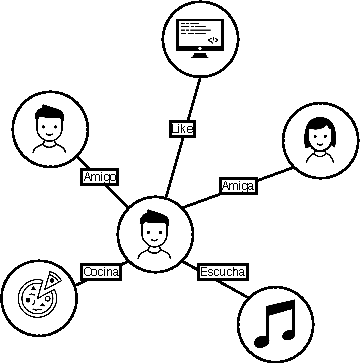
\includegraphics[scale=0.8]{Figures/facebook-graph.pdf}
	\caption{Grafo de relaciones en Facebook.}
	\label{fig:facebook-graph}
\end{figure}

Por otro lado, también muy cercano a la vida cotidiana de las personas, se encuentran las redes de telecomunicaciones, figura \ref{fig:teleco-graph}, que interconectan todos los aparatos eletrónicos, que de una manera u otra se comunicación entre ellos, y las redes de metro, figura \ref{fig:metro-graph}, que permiten el movimiento de las personas en la ciudad y pueden ser estudiadas por uso, localización, etcétera.

\begin{figure}[H]
	\begin{minipage}[b]{0.5\linewidth}
			\centering
			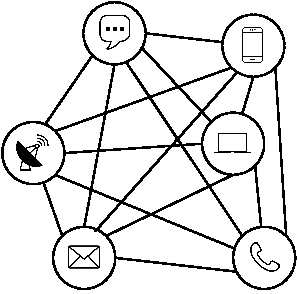
\includegraphics[scale=0.8]{Figures/teleco-graph.pdf}
			\caption{Grafo de telecomunicaciones.}
			\label{fig:teleco-graph}
	\end{minipage}
	\hspace{0.5cm}
	\begin{minipage}[b]{0.5\linewidth}
		\centering
		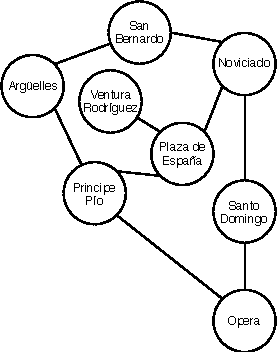
\includegraphics[scale=0.8]{Figures/metro-graph.pdf}
		\caption{Grafo sección del metro de Madrid.}
		\label{fig:metro-graph}
	\end{minipage}
\end{figure}

Y por último, otra representación de grafo, es el de las moléculas y los enlaces químicos \cite{grafo-molecula}, que se pueden representar como en la figura \ref{fig:molecula-graph}.

 \begin{figure}[H]
	\centering
	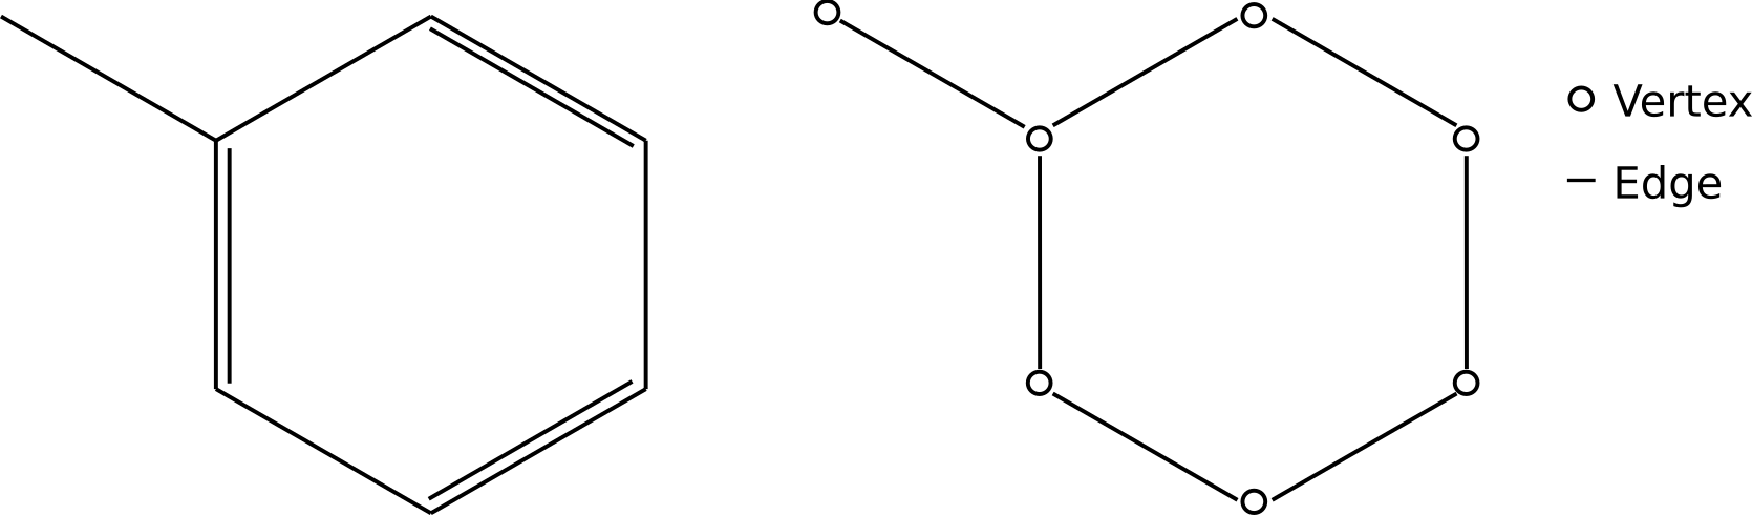
\includegraphics[scale=0.3]{Figures/molecula-graph.pdf}
	\caption{Representación estándar y en grafo de la molécula del Tolueno.}
	\scriptsize Fuente: https://www.blopig.com/blog/2019/01/graph-based-methods-for-cheminformatics
	\label{fig:molecula-graph}
\end{figure}

Estos ejemplos, tienen en común las conexiones entre todos los nodos que forman su estructura de grafo, y son muchas las aplicaciones e información que se obtiene de ellos como, nuevas terapias \cite{top-molec}, visión computacional y reconocimiento de patrones \cite{mcp-compVision}, análisis del mercado bursátil para conocer nuevas formas de predicción de éxito en inversiones \cite{vid-graf-ai}.

Por todo esto, es muy importante tratar los datos de forma adecuada y responsable, así como las relaciones entre ellos eficientemente. Para ello se han creado incluso base de datos orientadas a grafos, como es el caso de Neo4j \footnote{https://neo4j.com/}, con el fin de entender las relaciones y así poder hallar nuevas técnicas y más posibilidades para afrontar problemas y resolverlos de una manera mucho más ágil.


\section{Conceptos previos}
Para comprender mejor todas las explicaciones que se van a exponer a lo largo del documento, se describen a continuación los conceptos más importantes.

\subsection{Optimización combinatoria}
La optimización combinatoria es el área, dentro de las matemáticas aplicadas, que se encarga de maximizar o minimizar una función en un espacio de soluciones, el cuál debe ser finito. Los problemas que pertenecen a este área tienen en común la dificultad de encontrar soluciones factibles, puesto que existen muchas posibles y alguna de estas es óptima.\\
Algunos casos conocidos son el problema de la mochila\footnote{https://www.sciencedirect.com/topics/computer-science/knapsack-problem} o el problema del vendedor viajero\footnote{https://www.sciencedirect.com/topics/computer-science/travelling-salesman-problem}. Estos problemas tienen un planteamiento sencillo pero son difíciles de solucionar, y mediante ciertos algoritmos, como se explicará en la sección \ref{sec:heu-meta}, se pueden obtener soluciones factibles en tiempos de cómputo reducidos.\\
En la actualidad es un campo con un gran crecimiento ya que ``muchos de los problemas de la vida real pueden ser formulados mediante optimización combinatoria'' \cite{opt-comb-rg}.

\subsection{Heurística y Metaheurística}
\label{sec:heu-meta}
Se define heurística, según el Diccionario de la Real Academia de la Lengua Española \cite{rae-heuristica}, como ``técnica de la indagación y del descubrimiento'' y ``en algunas ciencias, manera de buscar la solución de un problema mediante métodos no rigurosos, como por tanteo, reglas empíricas, etc.''. Aplicándolo a temas científicos se define como el proceso de creación de medios, estrategias y principios para alcanzar un objetivo eficaz al problema dado \cite{conceptodef-heuristica}. El término heurística fue acuñado por George Polya en su libro ``How to Solve It'' \cite{gpolya-book-1}, más tarde traducido a ``Cómo plantear y resolver problemas'' \cite{gpolya-book-2}.

Añadiendo al término heurística el prefijo ``meta'', procedente del griego que significa ``más allá'' o ``nivel superior'', se puede definir metaheurística como el conjunto de procedimientos heurísticos combinados para obtener una solución a un problema que no tiene un algoritmo heurístico específico o su aplicación es ineficiente \cite{wiki-metaheuristica}. Este término lo acuñó Fred Glover en sus trabajos sobre búsqueda tabú en 1986 \cite{fred-glover}.

Existen una gran variedad de algoritmo metaheurísticos que se pueden clasificar de diferentes maneras según el enfoque, en la figura \ref{fig:clasif-metahs} se muestra una posible clasificación.

\begin{figure}[H]
	\centering
	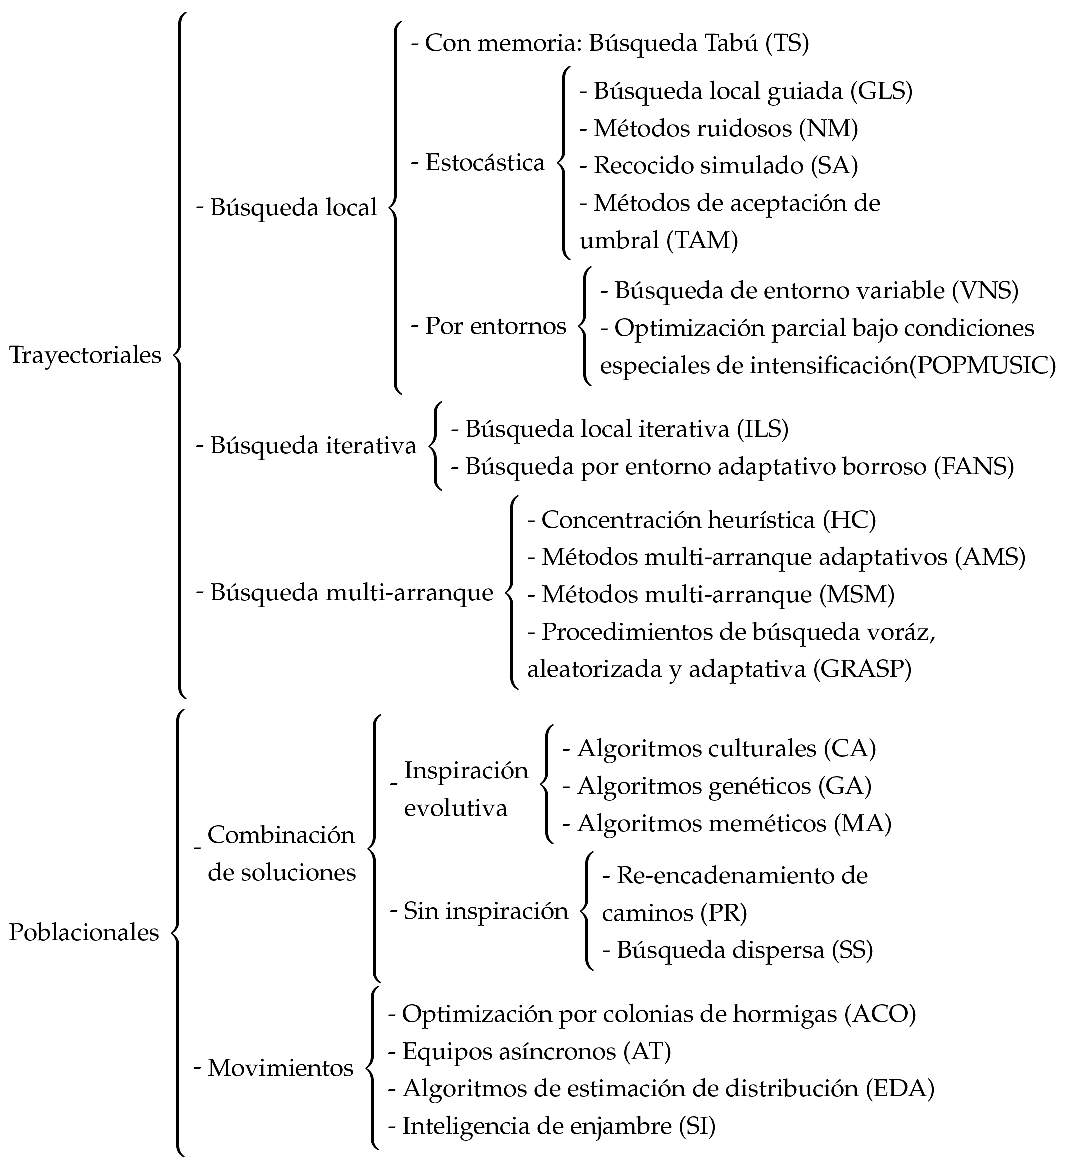
\includegraphics[scale=0.84]{Figures/diagrama-meta.pdf}
	\caption{Clasificación de metaheurísticas}
	\label{fig:clasif-metahs}
\end{figure}
%\begin{figure}[H]
%	\diagram{Trayectoriales}{
%		- \diagram{Búsqueda local}{
%			- Con memoria: Búsqueda Tabú (\gls{TS})\\ 
%			- \diagram{Estocástica}{
%				- Búsqueda local guiada (\gls{GLS}) \\ 
%				- Métodos ruidosos (\gls{NM}) \\ 
%				- Recocido simulado (\gls{SA})\\
%				- Métodos de aceptación de\\ umbral (\gls{TAM})
%			}\\
%			- \diagram{Por entornos}{
%				- Búsqueda de entorno variable (\gls{VNS})\\
%				- Optimización parcial bajo condiciones\\ especiales de intensificación(\gls{POPMUSIC})
%			}\\
%		}\\
%		- \diagram{Búsqueda iterativa}{
%			- Búsqueda local iterativa (\gls{ILS})\\
%			- Búsqueda por entorno adaptativo borroso (\gls{FANS})
%		}\\
%		- \diagram{Búsqueda multi-arranque}{
%			- Concentración heurística (\gls{HC})\\
%			- Métodos multi-arranque adaptativos (\gls{AMS})\\
%			- Métodos multi-arranque (\gls{MSM})\\
%			- Procedimientos de búsqueda voráz,\\ aleatorizada y adaptativa (\gls{GRASP})
%		}\\
%	}
%	\diagram{Poblacionales}{
%		- \diagram{Combinación\\de soluciones}{
%			- \diagram{Inspiración\\evolutiva}{
%				- Algoritmos culturales (\gls{CA})\\
%				- Algoritmos genéticos (\gls{GA})\\
%				- Algoritmos meméticos (\gls{MA})
%			}\\
%			- \diagram{Sin inspiración}{
%				- Re-encadenamiento de\\ caminos (\gls{PR})\\
%				- Búsqueda dispersa (\gls{SS})
%			}\\
%		}\\
%		- \diagram{Movimientos}{
%			- Optimización por colonias de hormigas (\gls{ACO})\\
%			- Equipos asíncronos (\gls{AT})\\
%			- Algoritmos de estimación de distribución (\gls{EDA})\\
%			- Inteligencia de enjambre (\gls{SI})
%		}\\
%	}
%\end{figure}

Dos conceptos a tener en cuenta en un algoritmo metaheurístico son la intensificación, que indica la exhaustividad con la que el algoritmo explora una región, y la diversificación, que indica como el algoritmo es capaz de explorar nuevas regiones del espacio de soluciones \cite{libro-metaheuristicas}.

\subsection{Clique}
\label{sec-clique}
El término clique se puede asemejar a un grupo de personas, las cuales serían los nodos o vértices de un grafo, a las que les unen los mismos intereses por algún tema en concreto, estas uniones serían las aristas que unen los nodos del grafo \cite{LUCE:1949}.

En teoría de grafos, un clique, es el subgrafo perteneciente a un grafo, en el cuál todos sus nodos o vértices son adyacentes entre sí, es decir, todo par de nodos o vértices están conectados mediante una arista. En términos matemáticos se describe como, dado un grafo $G = (V, E)$ donde $V$ indica el conjunto de vértices del grafo y $E$ indica el conjunto de aristas del grafo \cite{web-clique}, un clique $C$ se define como:
\[
C \subseteq V(G) ~ \wedge ~ u, v ~ \epsilon ~ C  \wedge  u  \neq v \Rightarrow u, v ~ \epsilon ~ E(G)
\]
Mostrandolo de una manera gráfica se indica en la figura  \ref{fig:graph} un grafo compuesto por el conjunto de nodos $V=\{A, B, C, D, E\}$.

\begin{figure}[H]
	\centering
	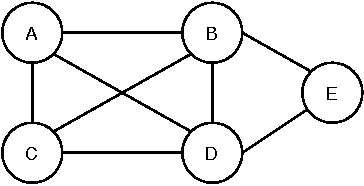
\includegraphics{Figures/graph.pdf}
	\caption{Diagrama de un grafo.}
	\label{fig:graph}
\end{figure}

En este grafo de ejemplo se encuentran los cliques con cardinalidad igual a 2 como se indican resaltado en negro en la figura \ref{fig:graph-cliques-2}.
\begin{figure}[H]
	\centering	
	\subfigure[Clique A-B]{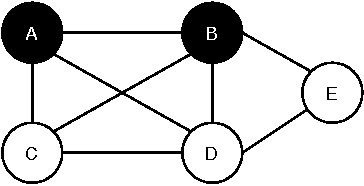
\includegraphics[width=0.275\textwidth]{Figures/graph-clique-AB.pdf}}
	\subfigure[Clique A-C]{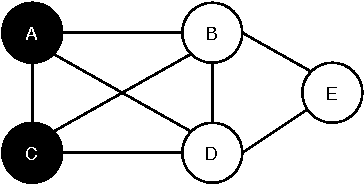
\includegraphics[width=0.275\textwidth]{Figures/graph-clique-AC.pdf}}
	\subfigure[Clique A-D]{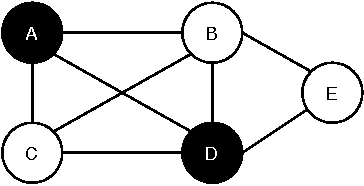
\includegraphics[width=0.275\textwidth]{Figures/graph-clique-AD.pdf}}
	\subfigure[Clique B-C]{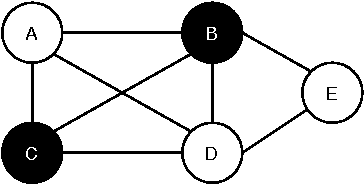
\includegraphics[width=0.275\textwidth]{Figures/graph-clique-BC.pdf}}
	\subfigure[Clique B-D]{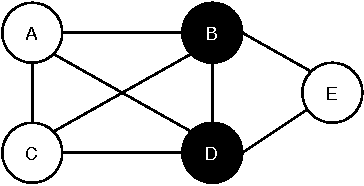
\includegraphics[width=0.275\textwidth]{Figures/graph-clique-BD.pdf}}
	\subfigure[Clique B-E]{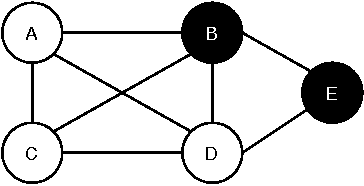
\includegraphics[width=0.275\textwidth]{Figures/graph-clique-BE.pdf}}
	\subfigure[Clique C-D]{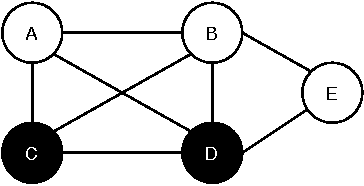
\includegraphics[width=0.275\textwidth]{Figures/graph-clique-CD.pdf}}
	\subfigure[Clique D-E]{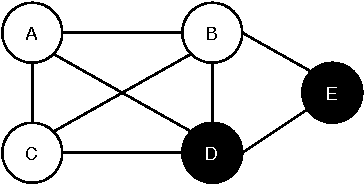
\includegraphics[width=0.275\textwidth]{Figures/graph-clique-DE.pdf}}
	\caption{Cliques de cardinalidad 2 del grafo.}
	\label{fig:graph-cliques-2}
\end{figure}
También se encuentran, como indica la figura \ref{fig:graph-cliques-3}, los cliques con cardinalidad igual a 3.
\begin{figure}[H]
	\centering	
	\subfigure[Clique A-B-C]{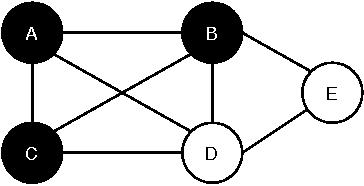
\includegraphics[width=0.275\textwidth]{Figures/graph-clique-ABC.pdf}}
	\subfigure[Clique A-B-D]{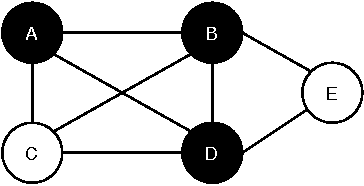
\includegraphics[width=0.275\textwidth]{Figures/graph-clique-ABD.pdf}}
	\subfigure[Clique A-C-D]{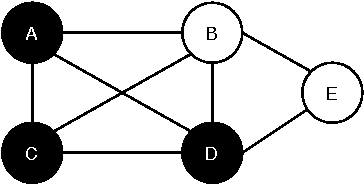
\includegraphics[width=0.275\textwidth]{Figures/graph-clique-ACD.pdf}}
	\subfigure[Clique B-C-D]{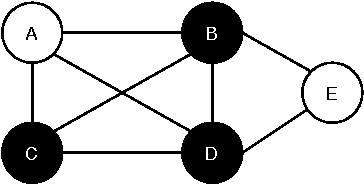
\includegraphics[width=0.275\textwidth]{Figures/graph-clique-BCD.pdf}}
	\subfigure[Clique B-D-E]{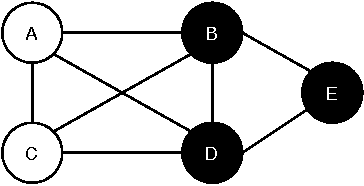
\includegraphics[width=0.275\textwidth]{Figures/graph-clique-BDE.pdf}}
	\caption{Cliques de cardinalidad 3 del grafo.}
	\label{fig:graph-cliques-3}
\end{figure}
Cabe destacar que los nodos, por si solos, también forman clique.

Una característica importante de un clique es que este puede ser máximo \cite{web-maximumclique}. Esto quiere decir que no se pueden añadir más nodos adyacentes que cumplan las restricciones necesarias para formar un clique, y a su vez, es el de mayor tamaño del grafo, como se muestra en la figura \ref{fig:max-clique}, a diferencia de un clique que se podría denominar simple  \cite{web-maximalclique}. 
\begin{figure}[H]
	\centering
	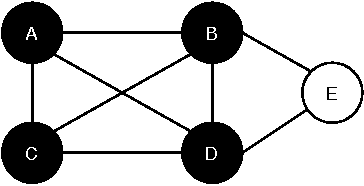
\includegraphics{Figures/graph-clique-max.pdf}
	\caption{Clique máximo del grafo.}
	\label{fig:max-clique}
\end{figure}
En este  caso, se obtiene $\omega(G) = 4$, donde $\omega$ denota el número de vértices del clique, su cardinalidad.

\section{Definición del problema}

\subsection{Problema del clique de ratio máximo}
\label{intro-problema}
Como se introdujo en la sección \ref{sec-clique}, el concepto clique es fundamental y muy estudiado, en concreto, la búsqueda del clique máximo dentro de un grafo. A este problema se le conoce como el problema del clique máximo o \gls{MCP} (Maximum clique problem), y es catalogado como un NP-completo.

En teoría de complejidad computacional, a los problemas denominados como NP, acrónimo de non-deterministic polynomial time o tiempo polinominal no determinista, se les conoce como el conjunto de problemas que se pueden resolver en un tiempo polinómico por una máquina de Turing no determinista. Esta clasificación, como se muestra en la figura \ref{fig:problemas-np}, también contiene todos los problemas de tipo P y de tipo NP-completos, como es el caso del problema del clique máximo.

\begin{figure}[H]
	\centering
	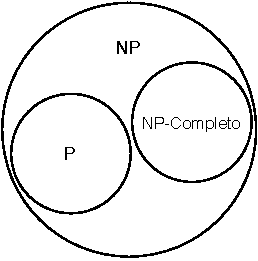
\includegraphics{Figures/problemas-np.pdf}
	\caption{Diagrama de problemas NP.}
	\label{fig:problemas-np}
\end{figure}

Una variante de este problema es el llamado problema del clique de peso máximo o \gls{MWCP} (Maximum Weight Clique Problem), en el que se asocia un peso no negativo a cada vértice, y cuyo objetivo es encontrar un clique con el máximo valor en la suma de los pesos de sus vértices. Este problema esta estrechamente ligado al problema tratado en este trabajo.\\
Otra variante, es la tratada en este trabajo y que se corresponde con el problema del clique de ratio máximo o \gls{MRCP} (Maximum Ratio Clique Problem) que trata de encontrar el subgrafo completo de ratio máximo. Este ratio se define como la proporción de la suma de los pesos no negativos asociados a los vértices del grafo como se indica a continuación:
\begin{equation*}
\frac{\sum_{i=1}^{n}p_ix_i}{\sum_{i=1}^{n}q_ix_i}
\end{equation*}
donde $p$ y $q$ son pesos no negativos asociados a cada vértice $i$, y $x$ se determina como:
\[
\diagram{$x_i=$}{
	1 : si el vértice $i$ forma parte de la solución. \\
	0 : en otro caso
}
\]

Como se expone en el modelo de ecuación \ref{eq:mrcp-max}, partiendo de un grafo simple no dirigido $G=(V, E)$, donde $V$ se asocia al conjunto de vértices pertenecientes al grafo, $\{v_1,\dots,v_n\}$, y $E$ es el conjunto de aristas que conectan los vértices del grafo, $\{(v_i,~v_j)\}$ tal que $i \neq j$ y $v_i,~v_j~\in V$, y suponiendo que los pesos asociados a cada vértice son positivos, se obtiene un clique máximo $\widehat{S}$, siempre y cuando se cumplan las restricciones \ref{eq:mrcp-rest1} - \ref{eq:mrcp-rest3}.

\begin{eqnarray}
\label{eq:mrcp-max} 
maximizar && f = \frac{\sum_{i=1}^{n}p_ix_i}{\sum_{i=1}^{n}q_ix_i} \\
\nonumber sujeto ~ a: \\
\label{eq:mrcp-rest1}
&& x_i + x_j \leqslant 1 : \forall (v_i, v_j) \notin E,~i \neq j,\\
\label{eq:mrcp-rest2}
&& \sum_{i=1}^{n}(a_ij)x_i ~ \geqslant 1 : \forall v_j \in V, \\
\label{eq:mrcp-rest3}
&& x_i \in {0,~1} : \forall v_i \in V.
\end{eqnarray}

El problema del clique de ratio máximo ha sido catalogado como un problema NP-difícil o NP-complejo como se indica en la figura \ref{fig:np-dificil}, por lo que no es posible obtener una solución factible por métodos heurísticos o exactos.

\begin{figure}[H]
	\centering
	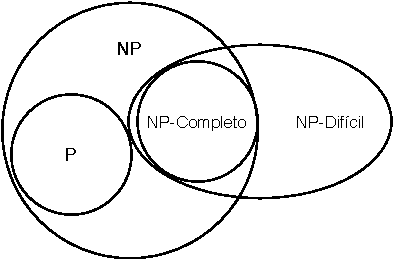
\includegraphics{Figures/problemas-np-hard.pdf}
	\caption{MRCP clasificado en los problemas NP-difícil.}
	\label{fig:np-dificil}
\end{figure}

\section{Estado del arte}
Si bien es cierto que no existe demasiada literatura al respecto, ya que se trata de un problema poco estudiado en comparación con el clásico problema de búsqueda de la clique máxima, \cite{mcp-batsyn}, \cite{mcp-ryp}, \cite{mcp-neuro}, o \cite{mcp-ants}, este análisis, y todo lo que rodea al mismo, ha sido documentado mediante la literatura que se explica a continuación. 

Un estudio muy cercano al tratado en este trabajo es el problema de la búsqueda del clique de peso máximo, en \cite{mwcp-ls} y \cite{mwcp-ml} se implementan algoritmos de búsqueda local, llamados SCCWalk y SCCWalk4L, en los que se hace uso del muestreo no determinista y el machine-learning para abordar el problema, eliminando variables de decisión que no formarían parte de una solución óptima.

En el documento desarrollado por Samyukta Sethuraman y Sergiy Butenko \cite{mrcp-Sethuraman:2015} se trata el problema desde tres puntos de vista, mediante el IBM CPLEX, para resolver el problema de manera lineal, la aplicación de la búsqueda binaria y el método de Newton.

En \cite{mrcp-moeni} se trata el problema basándose en el enfoque eficiente que dan las funciones de diferencia de convexos (DC) y sus algoritmos (DCA), que proveen resultados competitivos y a su vez introducen las desigualdades válidas, que ayudan a mejorar el tiempo computacional en la obtención de resultados de calidad al problema.

Cabe destacar entre todos los trabajos el de Dominik Goeke, Mahdi Moeini y David Poganiuch \cite{mrcp-GOEKE2017283} el cuál se ha tomado como referencia para realizar este trabajo. En este artículo, los autores parten de un punto de vista multi-arranque \gls{MSM}, añadiendo una búsqueda de vecindario variable \gls{VNS}, lo que permite obtener soluciones de gran calidad con un tiempo de computo menor.

%-------------------------------------------------------------------------------


% Chapter 2: Objectives

\chapter{Objetivos} % Main chapter title

\label{Chapter2}

%-------------------------------------------------------------------------------

En este apartado se indican los objetivos, tanto principales como secundarios, para la realización de este trabajo fin de grado:

\section{Objetivos principales}
\begin{itemize}
	\item Estudio y comprensión del problema de la búsqueda del clique de ratio máximo.
	\item Implementación del algoritmo metaheurístico GRASP para la resolución del problema.
\end{itemize}

\section{Objetivos secundarios}
\begin{itemize}
	\item Aprendizaje del lenguaje de programación Python para el desarrollo del algoritmo metaheurístico GRASP.
	\item Profundización y mejora en técnicas algorítmicas, de programación y de estructuras de datos para la realización de este trabajo fin de grado.
\end{itemize}

%-------------------------------------------------------------------------------

% Chapter 3: Algorithm description

\chapter{Descripción algorítmica} % Main chapter title

\label{Chapter3}

%-------------------------------------------------------------------------------
En este capítulo se describe el algoritmo metaheurístico utilizado, exponiendo todas sus características para la obtención de una solución al problema.

\section{Heurística y Metaheurística}
Se define heurística, según el Diccionario de la Real Academia de la Lengua Española \cite{rae-heuristica}, como ``técnica de la indagación y del descubrimiento'' y ``en algunas ciencias, manera de buscar la solución de un problema mediante métodos no rigurosos, como por tanteo, reglas empíricas, etc.''.

Aplicándolo a temas científicos se define como el proceso de creación de medios, estrategias y principios para alcanzar un objetivo eficaz al problema dado \cite{conceptodef-heuristica}, y en relación a esto, el término, fue acuñado por George Polya en su libro ``How to Solve It'' \cite{gpolya-book-1}, más tarde traducido a ``Cómo plantear y resolver problemas'' \cite{gpolya-book-2}.

Añadiendo al término heurística el prefijo ``meta'' procedente del griego, que significa ``más allá'' o ``nivel superior'', se puede definir metaheurística como el conjunto de procedimientos heurísticos combinados para obtener una solución, aunque no exacta si eficiente, a un problema que no tiene un algoritmo heurístico específico o su aplicación es ineficiente \cite{wiki-metaheuristica}. Este término lo acuño Fred Glover en sus trabajos sobre búsqueda tabú en 1986 \cite{fred-glover}.

Existen un gran variedad de algoritmo metaheurísticos que se pueden clasificar de diferentes maneras según el enfoque, en la figura \ref{fig:clasif-metahs} se muestra una de ellas basada en el número de soluciones.\\
\begin{figure}[H]
	\centering
\diagram{Trayectoriales}{
	- \diagram{Búsqueda\\local}{
		- Con memoria: Búsqueda Tabú (TS)\\ 
		- \diagram{Estocástica}{
			- Búsqueda local guiada (GLS) \\ 
			- Métodos ruidosos (NM) \\ 
			- Recocido simulado (SA)\\
			- Métodos de aceptación de\\ umbral (TAM)\\
		}\\
		- \diagram{Por \\entornos}{
			- Búsqueda de entorno variable (VNS)\\
			- Optimización parcial bajo condiciones\\ especiales de intensificación(POPMUSIC)\\
		}\\
	}\\
	- \diagram{Búsqueda\\iterativa}{
		- Búsqueda local iterativa (ILS)\\
		- Búsqueda por entorno adaptativo borroso (FANS\\
	}\\
	- \diagram{Búsqueda\\multi-arranque}{
		- Concentración heurística (HC)\\
		- (AMS)\\
		- Métodos multi-arranque (MSM)\\
		- Procedimientos de búsqueda voráz,\\ aleatorizada y adaptativa (GRASP)\\
	}\\
}
\diagram{Poblacionales}{
	- \diagram{Combinación\\de soluciones}{
		- \diagram{Inspiración\\evolutiva}{
			- Algoritmos culturales (CA)\\
			- Algoritmos genéticos (GA)\\
			- Algoritmos meméticos (MA)\\
		}\\
		- \diagram{Sin inspiración}{
			- Re-encadenamiento de\\ caminos (PR)\\
			- Búsqueda dispersa (SS)\\
		}\\
	}\\
	- \diagram{Movimientos}{
		- Optimización por colonias de hormigas (ACO)\\
		- Equipos asíncronos (AT)\\
		- Algoritmos de estimación de distribución (EDA)\\
		- Inteligencia de enjambre (SI)\\
	}\\
}
	\caption{Clasificación de metaheurísticas}
	\label{fig:clasif-metahs}
\end{figure}

Dos conceptos a tener en cuenta en algoritmo metaheurístico son la intensificación o explotación en una región, de modo que una alta intensificación hará que el algoritmo realice una búsqueda más exhaustiva en esa región, y la diversificación o exploración de nuevas regiones del espacio de soluciones \cite{libro-metaheuristicas}.

\section{Metaheurística GRASP\index{GRASP}}
El acrónimo GRASP se forma a partir de su siglas en inglés Greedy Randomized Adaptative Search Procedure o que en castellano es Procedimiento de búsqueda voráz aleatorizado y adaptativo, el término fue introducido por primera vez por Feo y Resende en 1995 en su artículo con el mismo nombre \cite{grasp-feo-resende}.

Este algoritmo se basa en el multi-arranque, dónde cada arranque es una iteración de un procedimiento que está constituido por dos partes bien diferenciadas, la fase constructiva, en la que se obtiene una solución de buena calidad, y una fase de mejora, en la que partiendo de la solución obtenida en la fase anterior, se intenta mejorar localmente \cite{libro-metaheuristicas}. 
En \cite{grasp-flightrecoveryproblem} \cite{grasp-parallel} \cite{grasp-weapon} \cite{grasp-empaquetado} \cite{grasp-ruta} \cite{grasp-vertex} se pueden encontrar diversos documentos en los que se tratan problemas aplicando la metaheurística GRASP.

En el algoritmo \ref{alg:grasp} se muestra el pseudocódigo de la metaheurística GRASP que se ha empleado para el desarrollo y obtención de una solución para este problema, dicho algoritmo se puede explicar aplicándolo al problema tratado de la siguiente manera:\\
Partiendo de un grafo $G=(V, E)$ donde $V$ son los vértices o nodos del grafo, y $E$ las aristas que unen estos nodos. Se toma un vértice $v$ aleatorio de entre los vértices del grafo. $v$ se incluye en la solución $S$ ya que cumple con las restricciones del problema, descritas en la sección XXX, a partir de $v$ se construye la lista de candidatos $CL$, definida como todos los nodos adyacentes a $v$ que forman parte de la lista de nodos del grafo de partida. A partir de este momento se toma un elemento de la lista de candidatos y con este se obtiene, mediante una función voráz el nodo con valor máximo y mínimo de esta función, con estos valores y un valor dado $\alpha$, que oscilará entre $0$ y $1$ y marca la aleatoriedad de la función de manera que si $\alpha$ es igual a 1 la función será menos aleatoria y se obtendría solo el mejor candidato, mientras que si es 0 la función es más aleatoria y se obtendrán todos los candidatos posibles, teniendo esto en cuenta, se obtiene el valor de $\mu$, el cuál pondrá el límite para la lista de candidatos restringida $RCL$, obtenida mediante la lista de candidatos $CL$ ordenada de mayor valor a menor valor tomando los primeros valores hasta alcanzar el valor de $\mu$. Tomando esta lista, se elegirá aleatoriamente un nodo de la misma, $u$, el cuál se añadirá a la lista solución $S$ y eliminándolo de la lista de candidatos junto con los nodos de la lista de candidatos que no son adyacentes a ese nodo. Este procedimiento será repetido hasta que la lista de candidatos este vacía, obteniéndose en ese momento la lista $S$ que conformará una solución.

\begin{algorithm}
	\SetAlgoLined
	$ v \gets rnd( V ) $ \\[0.2cm]
	$ S \gets \{ v \} $ \\[0.2cm]
	$ CL \gets \{u \in V : (u, v) \in E\} $ \\[0.2cm]
	\While{$|CL| \not= 0$}{
		$ \mathrm{g_{min}} \gets $ $ \smash{\displaystyle\min_{c \in CL}} \hspace{0.1cm} g(c) $ \\[0.2cm]
		$ \mathrm{g_{max}} \gets $ $ \smash{\displaystyle\max_{c \in CL}} \hspace{0.1cm} g(c) $ \\[0.2cm]
		$ \mu \gets  \mathrm{g_{max}} - \alpha ( \mathrm{g_{max}} - \mathrm{g_{min}} ) $ \\[0.2cm]
		$ RCL \gets \{ c \in CL : g(c) \geq \mu \}  $ \\[0.2cm]
		$ u \gets rnd (RCL) $ \\[0.2cm]
		$ S \gets \cup \hspace{0.1cm} \{ u \}$ \\[0.2cm]
		$ CL \gets CL \textbackslash \{ u \} \textbackslash \{ w : (u, w) \notin E \}$  \\[0.2cm]
	}
	\Return S
	\caption{Pseudocódigo algoritmo GRASP.}
	\label{alg:grasp}
\end{algorithm}

\subsection{Fase constructiva}

En esta fase se ha usado el algoritmo \ref{alg:const-voraz} el cuál es común a ambos constructivos y sólo se diferencian en como obtiene cada uno su mejor nodo a escoger para incluir en su solución, los cuales se definen a continuación.\\
\begin{algorithm}
	\SetAlgoLined
	$ S \gets \emptyset $  \\[0.2cm]
	$ Adyacentes \gets  SeleccionAdyacentes(nodo) $  \\[0.2cm]
	\While{$|Adyacentes| \not= 0$}{
		$ candidato \gets buscarMejor(adyacente) $  \\[0.2cm]
		\If{formaClique(candidato)}{
			$ Adyacentes \gets Adyacentes \cap SeleccionAdyacentes(candidato) $  \\[0.2cm]
			$ S \gets S \cup \{candidato\} $  \\[0.2cm]
		}\Else{
			$ Adyacentes \gets Adyacentes \textbackslash \{candidato\} $
		}
	}
	\Return S
	\caption{Contructivo voráz.}
	\label{alg:const-voraz}
\end{algorithm}

En primer lugar el algoritmo \ref{alg:const-voraz-ratio} para el constructivo que obtiene una solución mediante un algoritmo voraz buscando el mayor ratio de cada nodo adyacente al de partida.\\
\begin{algorithm}
	$ ratio \gets -1 $ \\[0.2cm]
	$ nodoElegido \gets NULO $ \\[0.2cm]
	\For{nodo}{
		$ ratioNodo \gets calcularRatio(nodo) $ \\[0.2cm]
		\If{ratioNodo >\hspace{0.1cm}  ratio}{
			$ ratio \gets ratioNodo $ \\[0.2cm]
			$ nodoElegido \gets nodo $ \\[0.2cm]
		}
	}
	\Return nodoElegido
	\caption{Pseudocódigo método buscarMejor de tipo ratio.}
	\label{alg:const-voraz-ratio}
\end{algorithm}


Y en segundo lugar, el algoritmo \ref{alg:const-voraz-ady} para el constructivo que obtiene una solución mediante un algoritmo voraz buscando el mayor número de vecinos de cada nodo adyacente al de partida.\\
\begin{algorithm}
	$ vecinos \gets -1 $ \\[0.2cm]
	$ nodoElegido \gets NULO $ \\[0.2cm]
	\For{nodo}{
		$ vecinosNodo \gets SeleccionAdyacentes(nodo) $ \\[0.2cm]
		\If{$ |vecinosNodo| $ >\hspace{0.1cm}  vecinos}{
			$ vecinos \gets |vecinosNodo|  $ \\[0.2cm]
			$ nodoElegido \gets nodo $ \\[0.2cm]
		}
	}
	\Return nodoElegido
	\caption{Pseudocódigo método buscarMejor de tipo adyacentes.}
	\label{alg:const-voraz-ady}
\end{algorithm}

\subsection{Fase de búsqueda}
Definición de la fase de búsqueda.


%-------------------------------------------------------------------------------


% Chapter 4: Design and Implementation

\chapter{Descripción informática} % Main chapter title

\label{Chapter4} % Reference

%-------------------------------------------------------------------------------

\section{Diseño}
aaa

\section{Implementación}
bbbb

\section{Metadología empleada}
Como afirma, Joaquín Alviz (2016) \cite{Reference1} "para poder contar con versiones del producto funcional que se puedan mostrar al cliente conformo se va mejorando y completando, es necesario contar con un enfoque ágil, flexible y con una retroalimentación constante", por esto para la elaboración de este trabajo final de grado se ha optado por seguir una metodología ágil de tipo iterativa e incremental, lo que permite evolucionar el proyecto progresivamente e ir adaptando los requisitos del cliente, en este caso los tutores del proyecto, en el menor tiempo posible, mejorando así la calidad del producto final con el menor esfuerzo.

Estas iteraciones e incrementos se han realizado durante todo el desarrollo del proyecto con un lapso de tiempo de aproximadamente 3 a 4 semanas entre ellas.

%-------------------------------------------------------------------------------


% Chapter 5: Results

\chapter{Resultados} % Main chapter title

\label{Chapter5} % Reference

%-------------------------------------------------------------------------------

En este capítulo se describen los diferentes recursos tanto hardware como software para la realización de este trabajo fin de grado, así como a partir de estos, se han obtenido los resultados para su posterior análisis.

\section{Recursos utilizados}
A continuación se detallará la máquina  y software para el desarrollo y procesado de las instancias para la comprobación del algoritmo, y las instancias utilizadas que describen diferentes casos y situaciones reales.

\subsection{Descripción de la máquina utilizada}
Para la realización de las diversas pruebas y procesado de las instancias de este problema, se ha utilizado una máquina con las siguientes características:

\begin{itemize}

\item \textbf{Procesador:} Intel Core i5 2,7 GHz
\item \textbf{Memoria RAM:} 8 GB 1867 Mhz DDR3
\end{itemize}

El desarrollo del código se ha realizado mediante el lenguaje de programación Python \footnote{https://www.python.org/}, en su versión 3.7.4, a través del IDE \footnote{Integrated Development Environment o entorno de desarrollo integrado.}, PyCharm \footnote{https://www.jetbrains.com/es-es/pycharm/} de JetBrains en su versión 2019.3.1.

\subsection{Instancias utilizadas}
Las instancias con las que se ha contado para comprobar la eficiencia del algoritmo desarrollado han sido proporcionadas por los estudios previos en los que se basa y compara este trabajo final de grado, estas, hacen referencia a diferentes conjuntos de grafos, tanto generados de manera aleatoria como obtenidos de diferentes fuentes de datos como precios del mercado de valores y turbinas de viento. A continuación se detallan los diferentes conjuntos:

\begin{itemize}
	
	\item \textbf{Conjuntos de tipo A y B:} Estos conjuntos son instancias de grafos generadas mediante una distribución de probabilidad uniforme, variando entre los 100 y los 500 nodos, así como la densidad del mismo que varía entre 45,78 \% y 53,64 \%.
	\item  \textbf{Conjunto de tipo C:} Los datos pertenecientes a las instancias de este tipo hacen referencia a datos de los precios del mercado de valores.
	\item  \textbf{Conjunto de tipo D:} Las instancias de este conjunto son datos para la construcción de turbinas de viento, donde cada nodo representa una localización de estas turbinas y sus pesos son la media de la velocidad del viento y el coste de contrucción de una turbina en ese punto.
	\item  \textbf{Conjunto de tipo E:} Estas instancias están extraídas del segundo y décimo DIMACS Implementation Challenge \footnote{http://dimacs.rutgers.edu/programs/challenge/}, donde cada nodo tiene un peso $\mathrm{p_{i} = 1}$ y un peso $\mathrm{q_{i} = 2}$. Adicionalmente se ha añadido un nodo más a cada instancia de este conjunto, el cual está conectado al resto de nodos de la misma, con un peso $\mathrm{p_{i} = 1}$ y un peso $\mathrm{q_{i} = 1}$, donde i es el número del nodo dentro de esa instancia.
	\item  \textbf{Conjunto de tipo F:} Estas instancias son las mismas que en el conjunto E pero en este caso los pesos de cada nodo son $\mathrm{p_{i} = i}$ y $\mathrm{q_{i} = |V| - i + 1}$, donde i es el número del nodo dentro de esa instancia.
	
	
\end{itemize}

%-------------------------------------------------------------------------------

\section{Análisis de los resultados}
Mostrar y comentar los resultados obtenidos.

%-------------------------------------------------------------------------------

% Chapter 6: Last Conclusions

\chapter{Conclusiones} % Main chapter title

\label{Chapter6} % Reference

%-------------------------------------------------------------------------------

En este capítulo se describen las conclusiones finales alcanzadas tras el desarrollo del proyecto, así como las lecciones aprendidas durante el mismo.

\section{Consecución de los objetivos}

Los objetivos establecidos al comienzo del proyecto son:

\begin{itemize}
	\item Estudio y comprensión del problema de la búsqueda del clique de ratio máximo.
	\item Estudio e implementación del algoritmo metaheurístico \gls{GRASP} para la resolución del problema.
\end{itemize}

Y por otro lado los objetivos secundarios:
\begin{itemize}
	\item Estudio de la importancia de los grafos en la vida real.
	\item Estudio de los distintos algoritmos metaheurísticos existentes.
	\item Estudio y comprensión de la complejidad computacional relacionada con la búsqueda de clique de ratio máximo.
	\item Aprendizaje del lenguaje de programación Python para el desarrollo del algoritmo metaheurístico \gls{GRASP}.
	\item Profundización y mejora en técnicas algorítmicas, de programación y de estructuras de datos para la realización de este trabajo fin de grado.
\end{itemize}

Estos objetivos se han cumplido de manera satisfactoria, puesto que se ha estudiado el estado del arte del problema del clique de ratio máximo para poder abordarlo, así como problemas relacionados como son el problema del clique de peso máximo (\gls{MWCP}) y el clásico problema del clique máximo (\gls{MCP}).
También se han estudiado las distintas familias en las que se categorizan los algoritmos metaheurísticos y en especial el algoritmo \gls{GRASP}.
Todo esto ha ayudado en la comprensión del problema y su posterior diseño e implementación.

%-------------------------------------------------------------------------------

\section{Conocimientos adquiridos}

El proceso de realización de este trabajo fin de grado ha supuesto la superación de diferentes retos los cuales han permitido ampliar conocimientos sobre el desarrollo de software y la gestión de un proyecto. También se ha profundizado en conceptos sobre algoritmia y estructuras de datos para obtener soluciones mejores y más eficientes al planteamiento de problemas de optimización. Destacando:

\begin{itemize}
  \item El aumento y mejora de conocimientos en el lenguaje de programación Python, usado para la implementación de este proyecto.
  \item La comprensión sobre conceptos de algoritmia y estructuras de datos, así como la mejora continua del código, enfocado en la resolución de problemas de optimización.
  \item Adquisición de conocimientos sobre heurísticas y metaheurísticas aplicadas a la resolución de problemas.
  \item Profundización en el uso de grafos en programación, así como la relación con el mundo real.
  \item El aprendizaje sobre \LaTeX, al utilizarlo para documentar el trabajo fin de grado.
\end{itemize}

\section{Líneas de desarrollo futuras}
En cuanto a las líneas de desarrollo futuras para este problema se describen algunas ideas como:

En primer lugar, un caso que ofrece un considerable aumento en el rendimiento del código, es la utilización de Cython\footnote{https://cython.org/} mediante pequeñas modificaciones en el código para ajustarlo a su lenguaje propio. Este compilador optimizado permite aumentar el  rendimiento de las funciones escritas en Python. Algunas de sus características son la unificación de la legibilidad del código escrito en Python con el rendimiento de C, y la interacción eficiente con grandes conjuntos de datos mediante NumPy\footnote{https://numpy.org/}.

Otra opción podría ser la implementación del procesado paralelo aprovechando el módulo $concurrent.futures$ que ofrece Python, este hace uso del módulo multiprocessing, por lo tanto no se ve afectado por el \gls{GIL}\footnote{https://docs.python.org/3/glossary.html?highlight=gil\#term-global-interpreter-lock} a diferencia del módulo multithreading, y permite crear un conjunto de procesos, mediante la función ProcessPoolExecutor, para ejecutar llamadas asíncronas. 

Esta opción se puede añadir para el cálculo de los valores a partir de la lista de todos los nodos candidatos, como se describió en la sección \ref{sec_metaGrasp} en el algoritmo \ref{alg:grasp}, con el fin de obtener los resultados de manera paralela, reduciendo considerablemente el tiempo de cómputo, ya que para instancias con una gran cantidad de nodos y una alta densidad este tiempo puede ser excesivo.

%-------------------------------------------------------------------------------


%-------------------------------------------------------------------------------
%	THESIS CONTENT - APPENDICES
%-------------------------------------------------------------------------------

%\appendix % Cue to tell LaTeX that the following "chapters" are Appendices

% Include the appendices of the thesis as separate files from the Appendices folder
% Uncomment the lines as you write the Appendices

% Appendix A

\chapter{Anexos} % Main appendix title

\label{Anexos} % For referencing this appendix elsewhere, use \ref{AppendixA}

\section{Resultados del experimento preliminar con el constructivo por adyacentes}
\label{anex:tabla_adys}

En la tabla \ref{table:ax-pre-ady} se muestran los resultados tras analizar las instancias seleccionadas para la experimentación preliminar mediante el constructivo por adyacentes, separada por el uso del algoritmo \gls{GRASP} y la posterior adición de la mejora, donde:
\begin{itemize}
	\item $f$: Indica el valor de la función objetivo calculado.
	\item c: Indica la cardinalidad del clique encontrado.
	\item t: Indica el tiempo total empleado en encontrar la solución en segundos.
	\item desv (\%): Indica la variación respecto al valor de la función objetivo mediante el algoritmo MS-VNS.
	\item \# Mejor: Indica si la solución obtenida mediante el algoritmo es mejor o no que la del trabajo anterior.
\end{itemize}

\begin{scriptsize}
	\pgfplotstabletypeset[
	multicolumn names,
	empty header,
	begin table=\begin{longtable},
		every first row/.append style={before row={
				\caption{Resultados de los experimentos preliminares con constructivo adyacentes.}
				\label{table:ax-pre-ady}\\\toprule
				\multicolumn{1}{c|}{\textbf{Instancias}} &
				\multicolumn{5}{c}{\textbf{GRASP}} &
				\multicolumn{5}{|c}{\textbf{GRASP y búsqueda local}} \\
				\multicolumn{1}{c|}{} & \multicolumn{1}{c}{\textbf{$f$}} & \textbf{c} &\textbf{t (sec)} & \textbf{desv(\%)} &\textbf{\#Mejor} & \multicolumn{1}{|c}{\textbf{$f$}} & \textbf{c} & \textbf{t (sec)} & \textbf{desv(\%)} & \textbf{\#Mejor} \\ \toprule
				\endfirsthead
				%
				\multicolumn{11}{c}
				{{\bfseries Tabla \thetable\ Continuación de la página anterior}} \\
				\toprule 
				\multicolumn{1}{c|}{\textbf{Instancias}} &
				\multicolumn{5}{c}{\textbf{GRASP}} &
				\multicolumn{5}{|c}{\textbf{GRASP y búsqueda local}} \\
				\multicolumn{1}{c|}{} & \multicolumn{1}{c}{\textbf{$f$}} & \textbf{c} &\textbf{t (sec)} & \textbf{desv(\%)} &\textbf{\#Mejor} & \multicolumn{1}{|c}{\textbf{$f$}} & \textbf{c} & \textbf{t (sec)} & \textbf{desv(\%)} & \textbf{\#Mejor} \\ \toprule
				\endhead
				\midrule \multicolumn{11}{r}{{Continúa en la siguiente página}} \\ \bottomrule
				\endfoot
				\midrule
				\multicolumn{11}{r}{{Concluido}} \\ \bottomrule
				\endlastfoot
		}},
		end table=\end{longtable},
	col sep=semicolon,
	string type,
	display columns/0/.style={postproc cell content/.append style={@cell content={\textbf{##1}}}},
	display columns/1/.style={column type={S}},
	display columns/2/.style={column type={c}},
	display columns/3/.style={column type={S}},
	display columns/4/.style={column type={S}},
	display columns/5/.style={column type={c}},
	display columns/6/.style={column type={S}},
	display columns/7/.style={column type={S}},
	display columns/8/.style={column type={S}},
	display columns/9/.style={column type={S}},
	display columns/10/.style={column type={c}},
	]{Results/pre-ady-fin.csv}
\end{scriptsize}

\section{Resultados del experimento preliminar con el constructivo por ratio}
\label{anex:tabla_ratio} % For referencing this appendix elsewhere, use \ref{AppendixA}

En la tabla \ref{table:ax-pre-ratio} se muestran los resultados tras analizar las instancias seleccionadas para la experimentación preliminar mediante el constructivo de ratio, separadas por el uso del algoritmo \gls{GRASP} y su posterior mejora, donde:
\begin{itemize}
	\item $f$: Indica el valor de la función objetivo calculado.
	\item c: Indica la cardinalidad del clique encontrado.
	\item t: Indica el tiempo total empleado en encontrar la solución en segundos.
	\item desv (\%): Indica la variación respecto al valor de la función objetivo mediante el algoritmo MS-VNS.
	\item \# Mejor: Indica si la solución obtenida mediante el algoritmo es mejor o no que la del trabajo anterior.
\end{itemize}

\begin{scriptsize}
	\pgfplotstabletypeset[
	multicolumn names,
	empty header,
	begin table=\begin{longtable},
	every first row/.append style={before row={
			\caption{Resultados de los experimentos preliminares con constructivo ratio.}
			\label{table:ax-pre-ratio}\\\toprule
			\multicolumn{1}{c|}{\textbf{Instancias}} &
			\multicolumn{5}{c}{\textbf{GRASP}} &
			\multicolumn{5}{|c}{\textbf{GRASP y búsqueda local}} \\
			\multicolumn{1}{c|}{} & \multicolumn{1}{c}{\textbf{$f$}} & \textbf{c} &\textbf{t (sec)} & \textbf{desv(\%)} &\textbf{\#Mejor} & \multicolumn{1}{|c}{\textbf{$f$}} & \textbf{c} & \textbf{t (sec)} & \textbf{desv(\%)} & \textbf{\#Mejor} \\ \toprule
			\endfirsthead
			%
			\multicolumn{11}{c}
			{{\bfseries Tabla \thetable\ Continuación de la página anterior}} \\
			\toprule 
			\multicolumn{1}{c|}{\textbf{Instancias}} &
			\multicolumn{5}{c}{\textbf{GRASP}} &
			\multicolumn{5}{|c}{\textbf{GRASP y búsqueda local}} \\
			\multicolumn{1}{c|}{} & \multicolumn{1}{c}{\textbf{$f$}} & \textbf{c} &\textbf{t (sec)} & \textbf{desv(\%)} &\textbf{\#Mejor} & \multicolumn{1}{|c}{\textbf{$f$}} & \textbf{c} & \textbf{t (sec)} & \textbf{desv(\%)} & \textbf{\#Mejor} \\ \toprule
			\endhead
			\midrule \multicolumn{11}{r}{{Continúa en la siguiente página}} \\ \bottomrule
			\endfoot
			\midrule
			\multicolumn{11}{r}{{Concluido}} \\ \bottomrule
			\endlastfoot
	}},
	end table=\end{longtable},
	col sep=semicolon,
	string type,
	display columns/0/.style={postproc cell content/.append style={@cell content={\textbf{##1}}}},
	display columns/1/.style={column type={S}},
	display columns/2/.style={column type={c}},
	display columns/3/.style={column type={S}},
	display columns/4/.style={column type={S}},
	display columns/5/.style={column type={c}},
	display columns/6/.style={column type={S}},
	display columns/7/.style={column type={S}},
	display columns/8/.style={column type={S}},
	display columns/9/.style={column type={S}},
	display columns/10/.style={column type={c}},
	]{Results/pre-ratio-fin.csv}
\end{scriptsize}

\section{Resultados del experimento final}
\label{anex:tabla_final} % For referencing this appendix elsewhere, use \ref{AppendixA}

En la tabla \ref{table:ax-exp-final} se muestran los resultados tras analizar todas las instancias durante la experimentación final, donde:
\begin{itemize}
	\item $f$: Indica el valor de la función objetivo calculado.
	\item c: Indica la cardinalidad del clique encontrado.
	\item t: Indica el tiempo total empleado en encontrar la solución en segundos.
	\item desv(\#): Indica la variación respecto al valor de la función objetivo en la que se ha basado este trabajo.
	\item \#Mejor: Indica si la solución obtenida mediante el algoritmo es mejor o no que la del trabajo anterior.
\end{itemize}

\begin{footnotesize}
	\pgfplotstabletypeset[
	empty header,
	begin table=\begin{longtable},
		every first row/.append style={before row={%
				\caption{Resultados del experimento final.}
				\label{table:ax-exp-final}\\\toprule
				\textbf{Instancias} &\textbf{$f$} &\textbf{c} &\textbf{t (sec)} &\textbf{desv(\%)} &\textbf{\#Mejor} \\ \toprule    
				\endfirsthead
				\multicolumn{6}{c}%
				{{\bfseries Tabla \thetable\ Continuación de la página anterior}} \\
				\toprule 
				\textbf{Instancias} &\textbf{$f$} &\textbf{c} &\textbf{t (sec)} &\textbf{desv(\%)} &\textbf{\#Mejor} \\ \toprule    
				\endhead
				\midrule \multicolumn{6}{r}{{Continúa en la siguiente página}} \\ \bottomrule
				\endfoot
				\midrule
				\multicolumn{6}{r}{{Concluido}} \\ \bottomrule
				\endlastfoot
		}},
		end table=\end{longtable},
	col sep=semicolon,
	string type,
	display columns/0/.style={postproc cell content/.append style={@cell content={\textbf{##1}}}},
	display columns/1/.style={column type={S}},
	display columns/3/.style={column type={S}},
	display columns/4/.style={column type={S}},
	]{Results/tabla-final.csv}
\end{footnotesize}

%-------------------------------------------------------------------------------
%\include{Appendices/AppendixB}
%\include{Appendices/AppendixC}

%-------------------------------------------------------------------------------
%	THESIS CONTENT - CONCEPTS INDEX
%-------------------------------------------------------------------------------

\printindex

%-------------------------------------------------------------------------------
%	BIBLIOGRAPHY
%-------------------------------------------------------------------------------

\printbibliography[heading=bibintoc]

%-------------------------------------------------------------------------------

\end{document}
